\chapter{Key concept--spatial point processes}


\section{A spatial point pattern}
% kleines Beispiel durchziehen
%David's data

Refer to Figure \ref{fig:rainpattern2}, which shows the spatial pattern formed by rainforest trees in a tropical rainforest in XXX. 

\begin{figure}
\centering
%\includegraphics[width=0.3\textwidth]{complete}
%\includegraphics[width=0.6\textwidth]{sealsscotland}
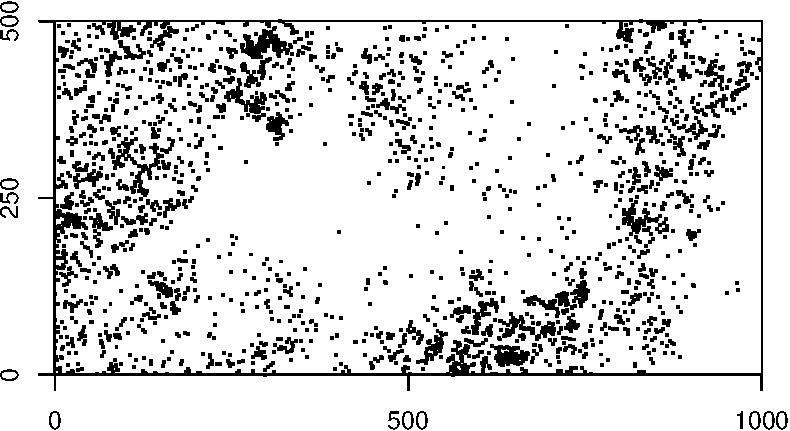
\includegraphics[width=0.6\textwidth]{rain_pattern}
\caption{\label{fig:rainpattern2} Rainforest trees...}
\end{figure}

It has some structure to it -- there are areas where we find more trees than in other areas, i.e.\ the density of trees varies in space. There is an interest in understanding why this is the case- and hence a study aim could be to understand the spatial structure formed by the locations of trees in space.
This is what point processes do -- they describe and model the spatial structure of 
 
\section{Spatial point processes--intuition}
Model location of objects in space.

\subsection{The intensity}
Initially one might want to understand how the density of trees varies in space, i.e.\ get a quantitative description of the number of individuals in space.

\subsection{Relationship to covariates}

\subsection{Marked point processes}

However, by just treating each individual simply as a point -- and hence assuming that all individuals are the same -- may still appear too simplistic. In many ecological data sets, in addition to spatial location further information associated with each individual is available. These data may take on many different forms and may be qualitative (age class, species) or quantitative (size or age) and are referred to as \textbf{marks}.  Note that we conceptionally distinguish between (spatial) covariates and marks. Spatial covariates take on values in continuous space -- even if they cannot be measured everywhere in space. Marks are properties of the objects represented by the points. As such marks can only take on values in a location where an object is present -- it does not make sense to consider the height of a tree in a location where there is no tree. The discussions throughout the book will make it clear why this distinction is relevant and not only a formal one.

We will see through the case studies in Chapter 5-9 that very different types of questions may be addressed with different types of marked point pattern data. For instance, in the context of qualitative marks multi-type patterns may refer to individuals from different species. Here, one is often interested in understanding the co-occurrence of the different species  in space.  In Chapter 5 we discuss several approaches to a multi-type point pattern such as the the pattern in  Figure \ref{chap1:fig3} which shows the locations of the tree species \textit{Protium Tenuifolium} that we have already met in  Figure \ref{chap1:fig2} along with another species \textit{Tabernaemontana arborea}.
\begin{figure}[h]
\begin{center}
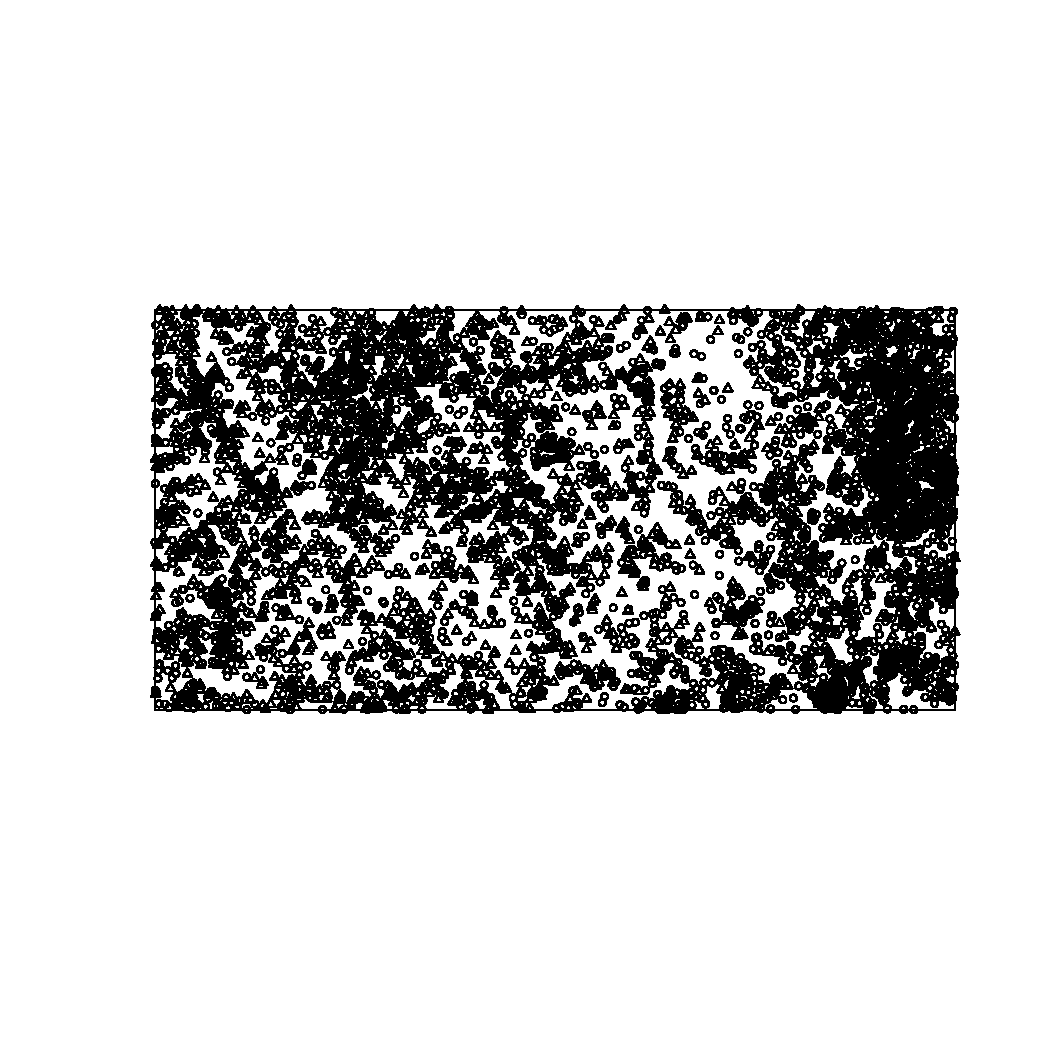
\includegraphics[width= 0.6\textwidth, angle= 0]{multitype}
\end{center}
\caption{The locations of 4294 trees of the species \textit{Protium Tenuifolium} (circles) and of 2213 trees of the species \textit{Tabernaemontana arborea} (triangles) in a 50 ha plot on Barro Colorado Island, Panama.}
%and a plot of the soil variable}
\label{chap1:fig3}
\end{figure}

In the context of quantitative marks one is often interested in assessing if the marks are related to the properties of the pattern itself. For example, trees may be smaller in areas where tree density is high but bigger where it is low. In addition, several marks may be available and these might depend on both the local intensity of the spatial pattern and on other marks. In Chapter 9 we discuss a model of eucalyptus trees (Figure \ref{chap1:fig4} (a)) for which chemical properties of the leaves (their palatability) are available  (Figure \ref{chap1:fig3} (b)), along with the frequency of use of the trees by koalas feeding on the leaves (Figure \ref{chap1:fig4} (c)). We assume that these two types of marks are dependent, and explicitly model the dependence along with the pattern itself, as well as the dependence of the pattern with the different marks. This type of model is computationally complex as it is a hierarchical model consisting of three (non-independent) levels with three separate likelihoods. Fitting a model of such a complexity with MCMC would be really time-consuming if not infeasible. We will show how such a model can be fitted with INLA in a straight forward way -- and will also show that the general structure of a hierarchical model with several dependent levels is a very versatile construction that may be used in many contexts, not only for marked point patterns.

 
\begin{figure}[!htb]
       \centering
    \begin{tabular}{c}
        \mbox{
            \subfigure[]{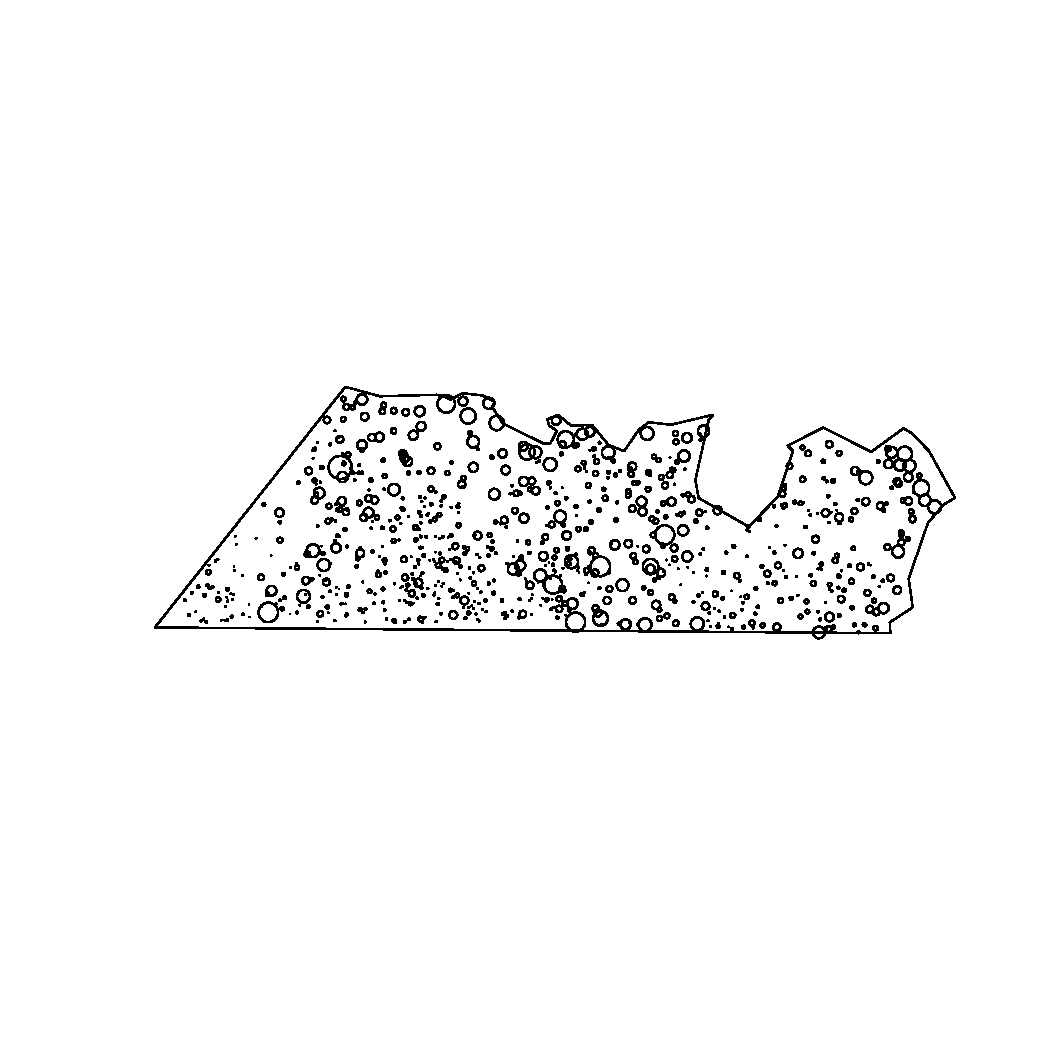
\includegraphics[width=10cm]{koala_food2_cut}}}\\
\mbox{
            \subfigure[]{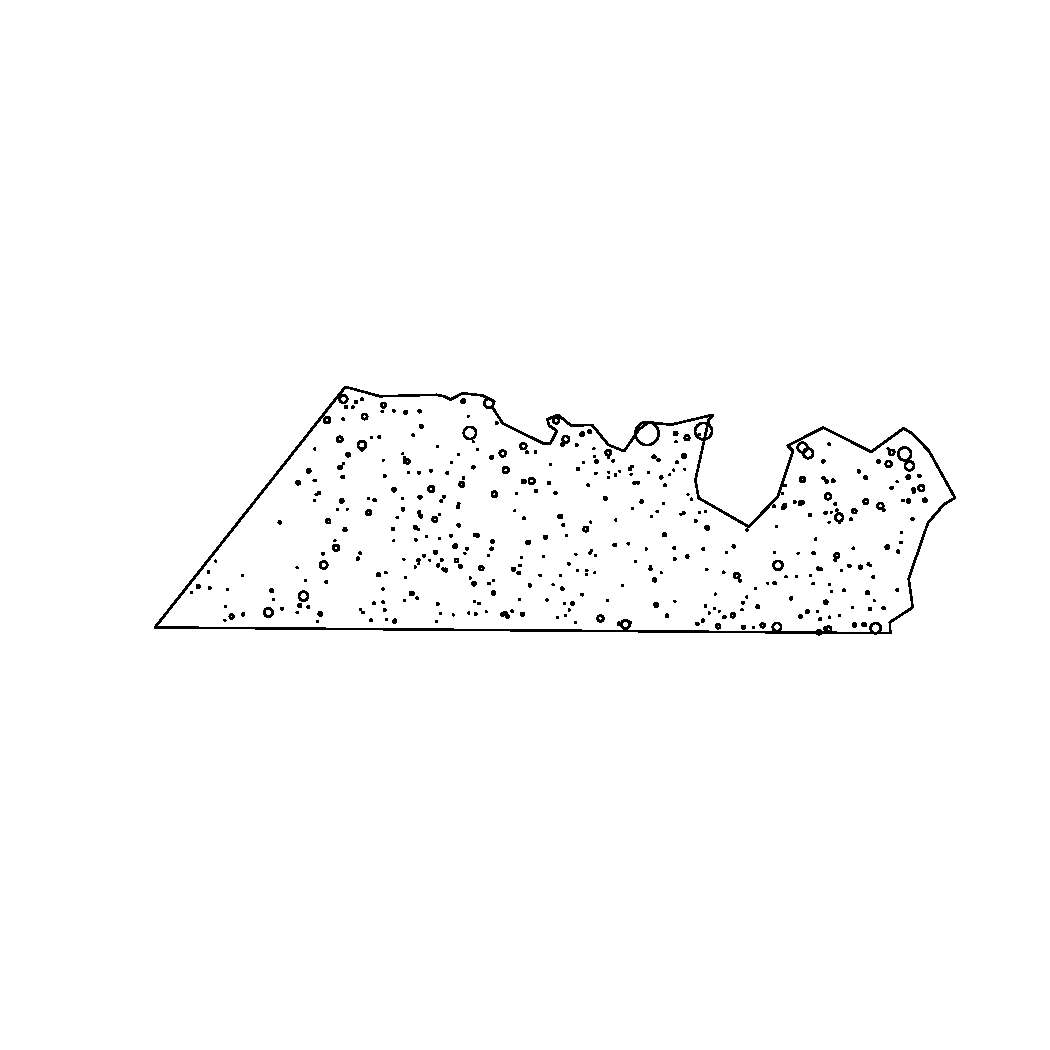
\includegraphics[width=10cm]{koala_freq2_cut}}}
    \end{tabular}
    \caption{Spatial pattern formed by the locations of the eucalyptus
        trees in the koala data set; the diameters of the circles
        reflect the value of the leaf marks (a) and the frequency
        marks (b) respectively.} 
\label{chap1:fig4}
\end{figure}

\section{Thinned point processes}

\subsection{Known thinning process}

\subsection{Unknown thinning process}

\section{Spatial point processes-- technical}
\subsection{Mathematical background}\label{ch1_maths}
The methodology developed for spatial point pattern data seeks to describe and analyse the patterns to infer information on the underlying mechanisms that generated them, i.e., a \textbf{spatial point pattern} formed by the spatial locations of objects in $d$-dimensional space, i.e.\ $\mathbf{x}=(x_1, \ldots, x_n)$, where $x_i \in \R^d, i = 1, \ldots, n$ and we typically have $d = 2$ or $d = 3$. 

%\janine{examples of patterns - properties -- thesis}

Technically, a spatial pattern is regarded as a realisation from a \textbf{random variable}, i.e.\  a stochastic structure that follows some distribution, referred to as a \textbf{spatial point process} $\mathbf{X}$. To understand this, recall the perhaps more familiar situation of data that are considered realisations from a theoretical random variable (or model) that follows, e.g., a normal distribution. In the context of spatial point patterns, the situation is complicated by the fact that all the points in the pattern together and the constellation that they form is a single observation (a single ``datum"). This implies that the random variable describing such a structure is bound to be a complicated mathematical object and hence to follow a rather complex distribution. This also implies that if an analysis is concerned with a single point pattern all information on this distribution has to be extracted from a single realisation\footnote{Ergodicity.}.

In this book, we focus on the practical analysis of spatial point patterns and refer the reader interested in the mathematical  details underlying spatial point processes to the relevant statistical literature.  However, to appreciate that a point pattern differs from a standard dataset and that it is indeed a complicated object note that a suitable random variable representing this data structure needs to capture the fact that the number of observed points is random. This implies that the mathematically complicated concept of a random measure has to be used. This in turn means that even the mathematics underlying a model for a data set with relatively simple structure such as the one in Figure \ref{chap1:fig1} are challenging. It is hence not surprising that within the history of mathematics these models have been described only relatively recently. Outside the statistical literature they have been considered very rarely but are becoming more popular these days.

A probability distribution (or model) familiar from non-spatial statistics assigns different probabilities to different realisations of a random variable -- realisations from a normal distribution are more likely to take on values that are close to the mean value but are less likely to take on values that are very different from the mean.  
Similarly, a specific \textbf{spatial point process model} characterises the properties of the random variable by assigning different probabilities to different realisations of the point process, only that now the realisations are point patterns. For instance, realisations from a model that reflects clustering are likely to be clustered and rather unlikely to be regular.  To achieve this, the mathematical formulation of a spatial point process model contains parameters.  These reflect the characteristics of the process and ultimately the characteristics of the generated patterns, i.e.\ characteristics such as clustering, regularity or randomness as well as homogeneity or inhomogeneity.  A number of different \textbf{classes} of spatial point process models with similar mathematical descriptions and properties have been formulated in the literature (see e.g.\ \cite{lieshout:00}, \cite{moeller:03}, \cite{stoystoy:94}).





